% El gradiente es normal a las equipotenciales
\documentclass[border=4pt]{standalone}
\usepackage{tikz}
\usetikzlibrary{arrows.meta, calc}
\begin{document}
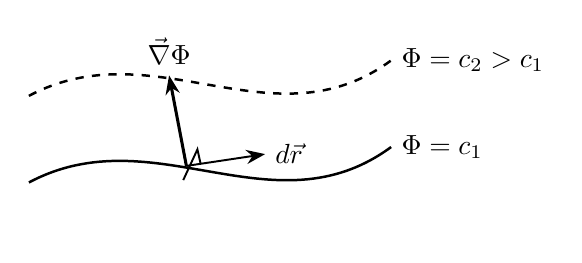
\begin{tikzpicture}[>={Stealth[length=2.4mm]}, line width=0.7pt]
  \draw[line width=0.9pt] (0,0.25) .. controls (1.6,1.1) and (3.1,-0.4) .. (4.6,0.7)
        node[right]{$\Phi=c_1$};
  \draw[line width=0.9pt, dashed] (0,1.35) .. controls (1.6,2.2) and (3.1,0.7) .. (4.6,1.8)
        node[right]{$\Phi=c_2>c_1$};
  \coordinate (P) at (2.0,0.46);
  % tangente (a lo largo de la curva) y gradiente (normal)
  \draw[->] (P)--($(P)+(1.0,0.15)$) node[right]{$d\vec r$};
  \draw[->, line width=1.1pt] (P)--($(P)+(-0.22,1.15)$) node[above]{$\vec\nabla\Phi$};
  \draw ($(P)+(0.18,0.03)$) -- ($(P)+(0.14,0.21)$) -- ($(P)-(0.04,0.18)$); % ángulo recto
\end{tikzpicture}
\end{document}
